\documentclass[answers,11pt]{exam}
\usepackage[spanish]{babel}
\usepackage[utf8]{inputenx}
\usepackage{fontenc}
\usepackage{textcomp}
\usepackage{lmodern,pifont}
\usepackage{graphicx}
\graphicspath{ {./images/} }
\usepackage{setspace}
\usepackage[dvipsnames]{color}
\usepackage{colortbl}
\usepackage{caption}
\usepackage{amsmath}
\usepackage[normalem]{ulem}

\newcommand\titexam[1]{\centering%
\fbox{\parbox{\textwidth}{\Large \sffamily \textbf{#1}}}\normalsize \vspace{1em}}

\newcommand\materia[1]{%
\parbox{\textwidth}{ \sffamily \textbf{\uline{#1}}}\vspace{1em}}


\newcommand\nombrefecha{%
Nombre y apellidos:\hrulefill
Fecha:\rule{3.5cm}{0.4pt}\vspace{0.5em}}

\renewcommand{\solutiontitle}{\noindent\textbf{Solución:}\par\noindent}
\pagestyle{empty}
\begin{document}
{\fontfamily{lmss}\selectfont

  %%%%%%%%%%%%%%%%%%%%%%%%%%%%%%%%%%%%%
  %% 
\titexam{UF0008 Instalaciones agrarias. Mantenimiento limpieza y desinfección}

\nombrefecha

\materia{Instalaciones y sus componentes}
\begin{questions}
  \question Señala cual de las siguientes es una ventaja en la producción de
    plantas en invernadero.
    \begin{checkboxes}
      \choice A. Mayor producción y obtener más de un ciclo de los cultivos
      durante un año
      \choice B. Requiere de personal especializado, tanto de experiencia
      práctica como de conocimientos teóricos
      \choice C. Mejor control de plagas y enfermedades
      \CorrectChoice D. Las respuestas A y C son correctas
    \end{checkboxes}
    
  \question De los siguientes materiales, señala cual NO es un material para la
    formación de cerramientos de un invernadero
    \begin{checkboxes}
      \choice A. Poliéster
      \choice B. Vidrio
      \choice C. Polimetacrilato de metilo
      \CorrectChoice D. Polietileno extruido
    \end{checkboxes}

  \question ¿Cual de las siguientes NO es una característica de un material de
    cerramiento?
    \begin{checkboxes}
      \choice A. Transparencia
      \choice B. Opacidad
      \CorrectChoice C. Resistencia a esfuerzos cortantes
      \choice D. Estanqueidad
    \end{checkboxes}

  \question ¿Qué tipo de factor influye en las tasas de crecimiento de manera
    determinante?
    \begin{checkboxes}
      \CorrectChoice A. Temperatura
      \choice B. Luminosidad
      \choice C. Humedad
      \choice D. Todas son correctas
    \end{checkboxes}

  \question Señala cual de los siguientes NO es un invernadero que se puede
    clasificar según la forma de su estructura
    \begin{checkboxes}
      \choice A. Invernadero plano o tipo parral
      \choice B. Invernadero asimétrico
      \choice C. Invernadero tipo tunel
      \CorrectChoice D. Invernadero de aluminio anodizado
    \end{checkboxes}
\newpage    
  \question La frase \emph{La temperatura, junto con la humedad ambiental, determina el
      desarrollo de diferentes plagas y enfermedades.} Es...
    \begin{checkboxes}
      \CorrectChoice A. Verdadera
      \choice B. Falsa
      \choice C. Verdadera, pero solo si tenemos en cuenta que el sistema de
      ventilación del invernadero funciona de manera deficiente
      \choice D. Falsa. Falta añadir la cantidad de radiación solar que recibe
      el invernadero
    \end{checkboxes}

  \question La luz desarrolla un papel fundamental en el ciclo vegetativo de las
    plantas. La luz influye en funciones tales como...
    \begin{checkboxes}
      \choice A. Fotosíntesis, fotoperiodismo, fototropismo y transpiración
      \choice B. Transpiración, floración y fructificación
      \choice C. Crecimiento y desarrollo de plagas y enfermedades
      \CorrectChoice D. Las respuestas A y B son correctas
    \end{checkboxes}

  \question ¿Como se llama al conjunto de procesos por el cual las plantas
    reaccionan según el número de horas de luz que reciben?
    \begin{checkboxes}
      \choice A. Fotosíntesis
      \choice B. Transpiración
      \CorrectChoice C. Fotoperiodo
      \choice D. Fototropismo
    \end{checkboxes}

  \question Según la cantidad de horas de luz que una planta puede recibir, ¿las
    plantas de día largo...?
    \begin{checkboxes}
      \choice A. Requieren de pocas horas de luz para florecer
      \CorrectChoice B. Requieren de pocas horas de oscuridad para florecer
      \choice C. Requieren de muchas horas de oscuridad para florecer
      \choice D. Ninguna es correcta
    \end{checkboxes}

  \question ¿El fenómeno por el cual las plantas tienen capacidad de dirigirse a
    la luz se llama?
    \begin{checkboxes}
      \choice A. Foto-morfogénesis
      \choice B. Fotosíntesis
      \choice C. Transpiración
      \CorrectChoice D. Fototropismo
    \end{checkboxes}
  \end{questions}
\newpage 
  %%%%%%%%%%%%%%%%%%%%%%%%%%%%%%%%%%%%%
  %% 
\titexam{UF0008 Instalaciones agrarias. Mantenimiento limpieza y desinfección}

\nombrefecha

\materia{Control ambiental}
\begin{questions}
  \question Las diferentes fases de un cultivo en un invernadero están
    condicionadas por cuatro factores ambientales o climáticos. Señala la opción
    correcta.
    \begin{checkboxes}
      \choice A. Topografía, humedad, temperatura y latitud
      \CorrectChoice B. Temperatura, humedad relativa, luz y concentración de
     $CO_2$
      \choice C. Temperatura, humedad del suelo, orientación y luminosidad
      \choice D. Topografía, viento dominante, humedad y tipo de invernadero
    \end{checkboxes}

  \question La frase: \emph{Podemos aumentar o disminuir la  temperatura de un
      invernadero ventilando, con sistemas de calefacción, refrigerando con
      agua o con mallas de sombreo.} ¿Es...?
    \begin{checkboxes}
      \CorrectChoice A. Verdadera
      \choice B. Verdadera pero teniendo en cuenta que solo podemos hacer esto
      con sistemas de control automáticos
      \choice C. Falsa
      \choice D. Es falsa ya que no se puede aumentar la temperatura de un invernadero ventilando
    \end{checkboxes}

  \question Para corregir los niveles de humedad ambiental en un invernadero,
    ¿qué métodos podemos emplear?
    \begin{checkboxes}
      \choice A. Manteniendo humedad en el suelo: mediante riegos o balsas de
      agua.
      \choice B. Enriquecer humedad en ambiente: mediante sistemas de aspersión,
      nebulización, etc
      \choice C. Disminuyendo la temperatura: ventilando, removiendo el aire o restando
      luminosidad
      \CorrectChoice D. Todas las respuestas son correctas
    \end{checkboxes}

  \question Los métodos para corregir los niveles de humedad consumen agua,
    ¿puedes indicar que métodos pueden usarse para ahorrar agua e influir en el
    nivel de humedad de un invernadero?
    \begin{checkboxes}
      \choice A. Sistemas de goteo
      \CorrectChoice B. Acolchados y sombreados
      \choice C. Sistemas de ventilación forzada
      \choice D. Sistemas de micro-nebulización
    \end{checkboxes}

  \question ¿Cual de los siguientes NO es un dispositivo para el control y automatización
    climáticos en un invernadero?
    \begin{checkboxes}
      \choice A. Higrómetro
      \CorrectChoice B. Interruptor diferencial
      \choice C. Fotostato
      \choice D. Analizador concentración de $CO_2$
    \end{checkboxes}

  \question ¿Cuando decimos que un conductor que lleva corriente toca otro cable
    o parte del circuito, nos referimos a que se ha producido un?
    \begin{checkboxes}
      \CorrectChoice A. Cortocircuito
      \choice B. Sobrecarga
      \choice C. Chispazo
      \choice D. Todas son correctas
    \end{checkboxes}

  \question ¿Como se llama un elemento de protección eléctrico que consta de un
    filamento de cobre que está diseñado para quemarse?
    \begin{checkboxes}
      \choice A. Interruptor magnetotérmico
      \choice B. Interruptor diferencial
      \choice C. Interruptor de toma de tierra
      \CorrectChoice D. Ninguna es correcta
    \end{checkboxes}

  \question ¿Como se llama el elemento de protección eléctrico que consta de
      dos partes, un electroimán y una lámina bimetálica?
      \begin{checkboxes}
        \choice A. Interruptor diferencial
        \choice B. Toma de tierra
        \CorrectChoice C. Interruptor magnetotérmico
        \choice D. Fusible
      \end{checkboxes}

  \question ¿Como se llama la estructura diseñada para guardar grano u otros
    materiales a granel?
    \begin{checkboxes}
      \CorrectChoice A. Silo
      \choice B. Cámara frigorífica
      \choice C. Invernadero
      \choice D. Ninguna es correcta
    \end{checkboxes}

  \question Señala que precauciones se deben tomar para realizar el mantenimiento
    de instalaciones agrícolas?
    \begin{checkboxes}
      \choice A. Seleccionar herramientas y útiles adecuados
      \choice B. Comprobar correcto funcionamiento de la maquinaria después del
      mantenimiento
      \choice C. Eliminación de residuos de productos y subproductos de las
      labores de mantenimiento
      \CorrectChoice D. Todas son correctas
    \end{checkboxes}
\end{questions}
  \newpage
%%%%%%%%%%%%%%%%%%%%%%%%%%%%%%%%%%
%%%%%%%%%%%%%%%%%%%%%%%%%%%%%%%%%%%%%%%%%

\titexam{UF0008 Instalaciones agrarias. Mantenimiento limpieza y desinfección}

\nombrefecha

\materia{Productos y equipos de limpieza. Prevención de riesgos}
\begin{questions}

  \question ¿Como se llama la lucha contra bacterias, virus, hongos, etc que se
    pueden desarrollar en las instalaciones agrícolas?
    \begin{checkboxes}
      \choice A. Limpieza
      \choice B. Desratización
      \choice C. Método de lucha activo
      \CorrectChoice  D. Desinfección
    \end{checkboxes}

  \question ¿Los productos químicos llamados desinfectantes generalmente son?
    \begin{checkboxes}
      \CorrectChoice A. Productos a base de compuestos clorados o amoniacales
      (lejía y amoniaco)
      \choice B. Productos a base de aceites esenciales
      \choice C. Productos a base de jabón y agua
      \choice D. Ninguna respuesta es correcta
    \end{checkboxes}

  \question A la acción de controlar las plagas presentes en la instalación
    tales como moscas, hormigas, cucarachas, etc, ¿como la llamamos?
    \begin{checkboxes}
      \choice A. Desratización
      \choice B. Desinfección
      \CorrectChoice C. Desinsectación
      \choice D. Limpieza
      \end{checkboxes}
  \question Los métodos de lucha para la desinsectación pueden ser medidas
    físicas, químicas y
    \begin{checkboxes}
      \choice A. Dispositivos de cierre
      \choice B. Colocación de mallas anti trips
      \CorrectChoice C. Biológicas
      \choice D. Ninguna respuesta es correcta
    \end{checkboxes}

  \question De las siguientes medidas señala la que NO es una medida física de
    lucha para la desinsectación
    \begin{checkboxes}
      \choice A. Colocar mosquiteras
      \CorrectChoice B. Colocación de trampas-cebo
      \choice C. Sellar grietas, oquedades y hendiduras
      \choice D. Extremar medidas de limpieza
    \end{checkboxes}
\newpage
  \question ¿Qué tipo de señales tienen forma triangular con fondo amarillo y
    bordes negros?
    \begin{checkboxes}
      \CorrectChoice A. Advertencia de peligro
      \choice B. De obligación
      \choice C. De prohibición
      \choice D. De equipos contra incendios
    \end{checkboxes}

  \question ¿Qué tipo de señales tiene forma redonda, pictograma negro sobre
    fondo blanco atravesado por una banda descendente de izquierda a derecha a
    45\textdegree{}?
    \begin{checkboxes}
      \choice A. Advertencia de peligro
      \choice B. De obligación
      \CorrectChoice C. De prohibición
      \choice D. De equipos contra incendios
    \end{checkboxes}

  \question ¿Que tipo de señales tienen forma redonda. Pictograma blanco sobre
    fondo azul (el azul deberá cubrir como mínimo el 50\% de la superficie de la
    señal).
    \begin{checkboxes}
      \choice A. Advertencia de peligro
      \choice B. De equipos contra incendios
      \choice C. De prohibición
      \CorrectChoice D. Ninguna es correcta
    \end{checkboxes}

  \question Los equipos de protección respiratoria los clasificamos en dos
    grandes grupos.
    \begin{checkboxes}
      \choice A. Mascarillas desechables y no desechables
      \CorrectChoice B. Equipos filtrantes y equipos aislantes
      \choice C. Equipos de línea de aire y equipos autónomos
      \choice D. De presión positiva y filtrantes
    \end{checkboxes}

  \question ¿Qué señala la imagen siguiente? (El pictograma es negro sobre fondo
    amarillo)
  \begin{figure}[h!]
    \centering
    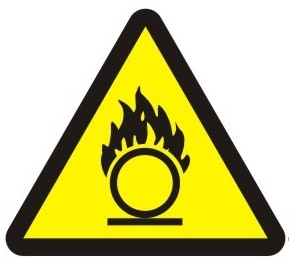
\includegraphics[scale= 0.6]{images/combustible.jpg}
  \end{figure}
  \begin{checkboxes}
    \CorrectChoice A. Peligro material combustible
    \choice B. Prohibido encender fuego
    \choice C. Peligro atrapamiento
    \choice D. Peligro de incendio
  \end{checkboxes}
\end{questions}
  \newpage
%%%%%%%%%%%%%%%%%%%%%%%%%%%%%%%%%%
%%%%%%%%%%%%%%%%%%%%%%%%%%%%%%%%%%%%%%%%%
\titexam{UF0009 Mantenimiento, preparación y manejo de tractores}

\nombrefecha

\materia{Tractor y equipo de tracción}

\begin{questions}
\question El tractor es una máquina que tiene diferentes aplicaciones en agricultura y selvicultura. Los diferentes trabajos que realiza los podemos clasificar en...
\begin{checkboxes}
\choice A. De excavación, de desbroce, de empuje y de arrastre
\CorrectChoice B. Estacionarios, de transporte, de arrastre, de empuje y combinados
\choice C. De limpieza y arrastre
\choice D. Ninguna es correcta
\end{checkboxes}

\question ¿En cuantas partes podemos dividir visualmente un motor de combustión interna? 
\begin{checkboxes}
\choice A. 4 partes. Carter, culata, filtros y volante de inercia
\choice B. 3 partes. Carter, cilindros y embrague 
\CorrectChoice C. 3 partes. Carter, bloque motor y tapa de culata
\choice C. 4 partes. Carter, culata, motor de arranque y radiador    
\choice D. 2 partes. Carter y bloque motor
\end{checkboxes}

\question Si en el cilindro de un motor diesel de 4t, encontramos las válvulas de admisión y escape cerradas, ¿en  qué tiempos y carrera puede estar el motor?
\begin{checkboxes}
\CorrectChoice A. Carrera ascendente de compresión o carrera descendente de expansión 
\choice B. Carrera ascendente de admisión o carrera descendente de escape
\choice C. Carrera descendente de expansión o carrera descendente de admisión
\choice D. Carrera ascendente de compresión o carrera ascendente de escape
\end{checkboxes}

\question El sistema de engrase de un motor de 4t, ¿es importante controlar la presión del sistema?
\begin{checkboxes}
\choice A. No se controla la presión del sistema de engrase
\CorrectChoice B. Si. Es muy importante y se controla mediante un manómetro o testigo luminoso
\choice C. El sistema de engrase del motor no necesita supervisión
\choice D. El sistema de engrase es importante para el motor pero no hay manera de controlarlo
\end{checkboxes}

\question ¿Generalmente que tipo de refrigeración lleva el motor de un tractor?
\begin{checkboxes}
\choice A. De aire
\choice B. De aire o de agua
\choice C. De ventilación forzada
\CorrectChoice D. De agua
\end{checkboxes}
\newpage 
\question ¿De que tipo de sistema de frenos estamos hablando si entre sus componentes se encuentran \emph{pastillas} y pinza?
\begin{checkboxes}
\CorrectChoice A. Sistema de frenos de disco
\choice B. Sistema de frenos de tambor
\choice C. Sistema de zapatas exterior
\choice D. Ningúna es correcta
\end{checkboxes}

\question  ¿Como se llama el dispositivo que transmite o interrumpe el giro del motor para dar movimiento al vehiculo?
\begin{checkboxes}
\CorrectChoice A. Embrague
\choice B. Diferencial
\choice C. Palier
\choice D. Ninguna de ella es correcta
\end{checkboxes}

\question ¿Podrías decir como se llama el armazón metálico sobre el que se sujetan las diferentes partes de un tractor?
\begin{checkboxes}
\choice A. Motor
\choice B. Enganche tri-puntal
\choice c. Toma de fuerza
\CorrectChoice D. Bastidor
\end{checkboxes}

\question Si un motor de combustión interna no tiene sistema de engrase, ¿qué tipo de motor es?
\begin{checkboxes}
\choice A. De un motor que utiliza \emph{gasoil} como combustible
\CorrectChoice B. Motor de dos tiempos
\choice C. Todos los motores tienen un sistema de engrase
\choice D. Ningúna es correcta
\end{checkboxes}

\question ¿Qué tipo de estructuras de protección antivuelco existen para tractores?
\begin{checkboxes}
\choice A. Solo cabinas
\CorrectChoice B. Bastidor de dos postes, bastidor de cuatro postes y cabina
\choice C. Bastidor de dos y cuatro postes
\choice D. Cabina cerrada
\end{checkboxes}
\end{questions}
\newpage 
%%%%%%%%%%%%%%%%%
%%%%%%%%%%%%%%%%%
\titexam{UF0009 Mantenimiento, preparación y manejo de tractores}
\nombrefecha

\materia{Mantenimiento y prevención}

\begin{questions}
\question ¿Qué tipo de mantenimiento tenemos que realizar para evitar riesgos y garantizar la seguridad del operador a la vez que reducimos costes innecesarios?
\begin{checkboxes}
\choice A. Mantenimiento correctivo
\choice B. Mantenimiento regular
\CorrectChoice C. Mantenimiento preventivo
\choice D. Ninguna es correcta
\end{checkboxes}

\question ¿Como se llama el intervalo de tiempo en el que in objeto puede cumplir correctamente la función para la que ha sido diseñado?
\begin{checkboxes}
\choice A. Tiempo de funcionamiento
\CorrectChoice B. Vida útil
\choice C. Vida de estimada de funcionamiento
\choice D. Todas son correctas
\end{checkboxes}

\question Para hacer una limpieza de bornes de batería, ¿cual es el orden en el que hay que retirar los cables para desconectarla?
\begin{checkboxes}
\CorrectChoice A. Primero el cable del borne negativo y despues el positivo
\choice B. Primero el positivo y despues el negativo
\choice C. Retiramos los dos a la vez
\choice D. No hay que retirar los cables para desconectarla, simplemente quitar las llaves del contacto
\end{checkboxes}

\question ¿Qué es recomendable hacer antes de poner en marcha un tractor que no conocemos y ponemos en funcionamiento por primera vez?
\begin{checkboxes}
\CorrectChoice A. Leer el manual del fabricante
\choice B. Comprobar niveles
\choice C. Comprobar en la hoja de vida el mantenimiento realizado
\choice D. Comprobar que no hay tornillos sueltos
\end{checkboxes}

\question ¿Cual es la principal operación que hay que realizar para  que la bomba de inyección no se estropee?
\begin{checkboxes}
\choice A. Poner gasolina de 98 octanos
\choice B. Poner aditivos al combustible
\CorrectChoice C. Cambiar el filtro de gasoil según las indicaciones del fabricante
\choice D. Llenar el tanque de combustible al final de cada jornada
\end{checkboxes}
\newpage 

\question ¿Cuales son las zonas de riesgo comunes a cualquier máquina agrícola?
\begin{checkboxes}
\choice A. Puntos de corte y cizallamiento
\CorrectChoice B. Engranajes, puntas y aristas de corte y cizallamiento, ejes y puntos giratorios de arrollamiento, puntos de arrastre, puntos de aplastamiento y las proyecciones
\choice C. Engranajes y puntos de arrastre
\choice D. Todas son correctas
\end{checkboxes}

\question La estructura anti-vuelco de un tractor, ¿imposibilita que un tractor pueda sufrir un vuelco?
\begin{checkboxes}
\choice A. Si. Están diseñadas para que impidan el vuelco de un tractor
\choice B. Si, pero han de emplearse medidas de seguridad complementarias como el cinturon de seguridad
\choice C. Si, pero solo si es una cabina
\CorrectChoice D. No. No están diseñados para impedir la posibilidad de vuelco, solo para minimizar la gravedad de las lesiones en caso de accidente
\end{checkboxes}

\question ¿Qué medidas de protección son adecuadas para los puntos de engranaje?
\begin{checkboxes}
\choice A. No operar la máquina sin que las protecciones de estos puntos no estén colocadas
\choice B. Conocer dichos puntos, localizarlos y evitar aproximarse a ellos cuando la máquina esté en funcionamiento
\choice C. No realizar ningúna intervención cuando la máquina o alguna de sus partes esté en movimiento
\CorrectChoice D. Todas son correctas
\end{checkboxes}

\question ¿Qué peligro señala el pictograma de la imagen?
\begin{figure}[h!]
    \centering
    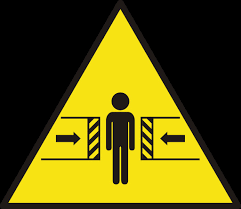
\includegraphics[scale= 0.8]{aplastamiento.png}
\end{figure}
\begin{checkboxes}
\choice A. Atrapamiento
\CorrectChoice B. Aplastamiento
\choice C. Corte
\choice D. Ningúna es correcta
\end{checkboxes}

\newpage
\question ¿Qué peligro señala el pictograma de la imagen?
\begin{figure}[h!]
    \centering
    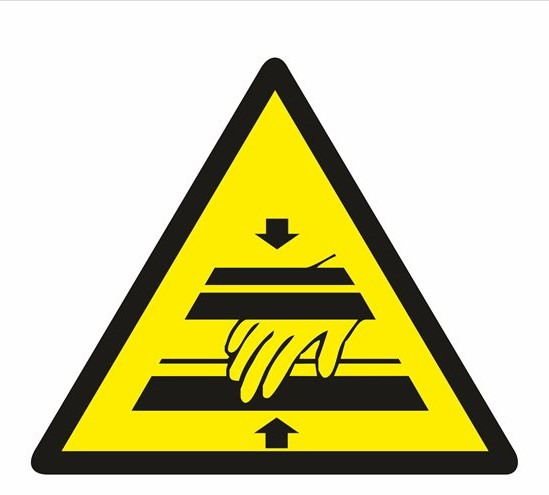
\includegraphics[scale= 0.6]{images/corte_mano.jpg}
\end{figure}
\begin{checkboxes}
\choice A. Atrapamiento
\choice B. Aplastamiento
\CorrectChoice C. Corte
\choice D. Ningúna es correcta
\end{checkboxes}
\end{questions}}
\end{document}

%%% Local Variables:
%%% mode: latex
%%% TeX-master: t
%%% End:
